\chapter{DL\,03 – Entscheidungsbaum}

\begin{myremark}
Der Entscheidungsbaum ist einer der \textbf{intuitivsten} ML-Algorithmen:
Er stellt Entscheidungen als Baumstruktur dar und ist leicht zu interpretieren.
\end{myremark}

\section{Grundidee}

\begin{mydefinition}[Entscheidungsbaum]
Ein \textbf{Entscheidungsbaum} teilt Daten schrittweise auf.
Jede \textbf{innere Knoten} stellt eine Frage (z.\,B. \enquote{Lernzeit > 6\,h?}),
jede \textbf{Kante} führt zu einer Teilmenge, und jedes \textbf{Blatt} gibt
die vorhergesagte Klasse an.
\end{mydefinition}

\begin{figure}[H]
    \centering
    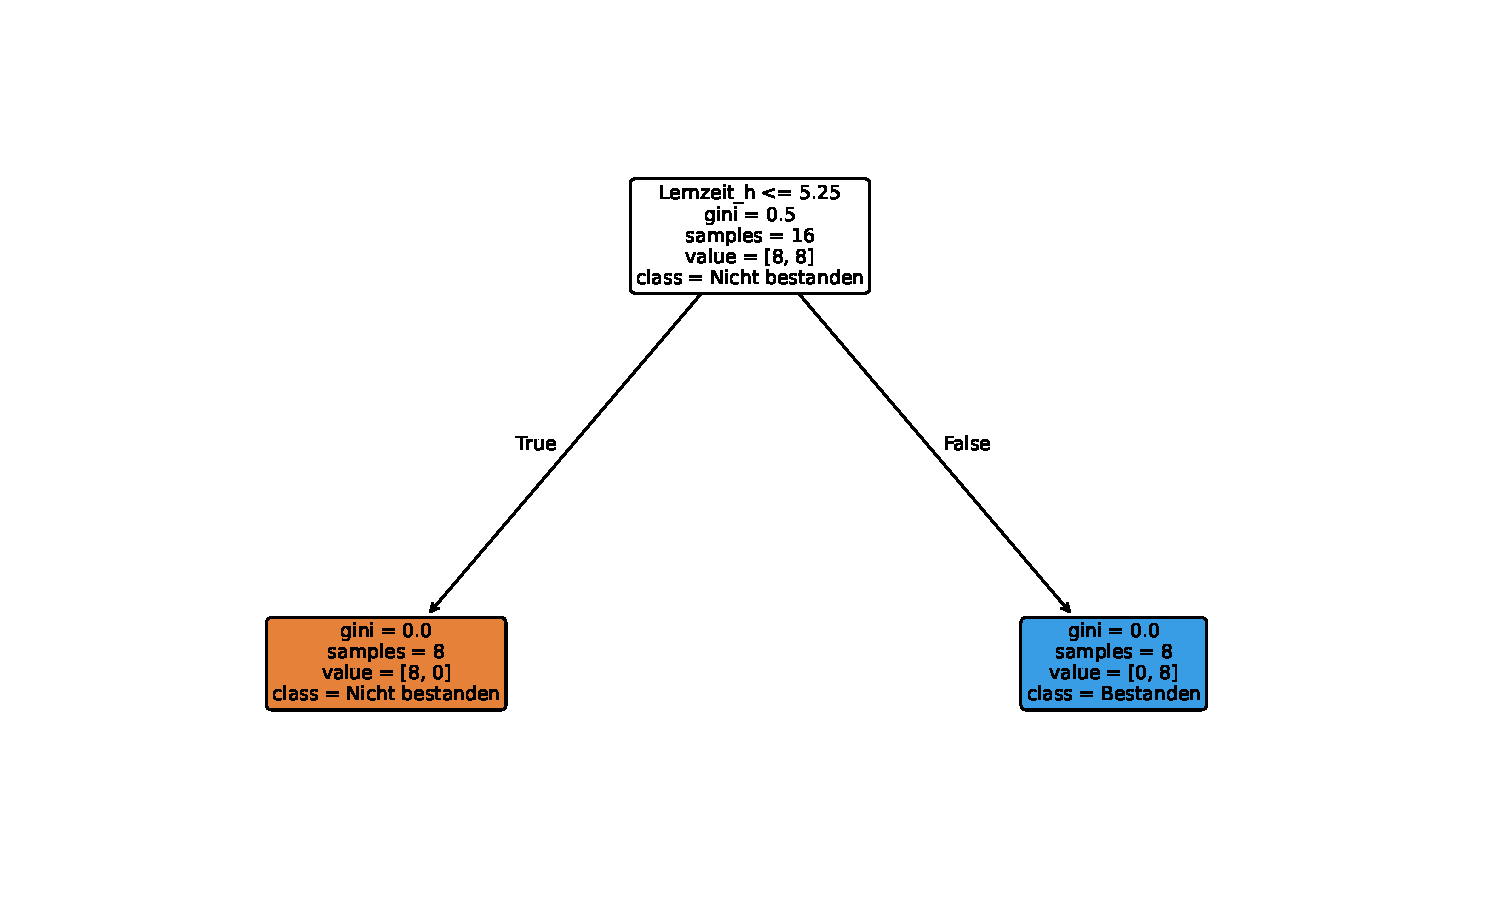
\includegraphics[width=0.8\textwidth]{Grundlagen_Info/15_KI_und_Algorithmen/Figures/decision_tree_structure.pdf}
    \caption{Beispiel eines Entscheidungsbaums}
    \label{fig:tree-15}
\end{figure}

\section{Wie lernt ein Baum?}

Ein Baum wählt an jedem Knoten jene Frage, die die Daten am besten aufteilt.
Als Gütemass wird häufig der \textbf{Gini-Koeffizient} verwendet:
\[
\text{Gini}(t) = 1 - \sum_{k} p_k^2
\]
wobei $p_k$ der Anteil der Klasse $k$ im Knoten $t$ ist.
Ein Gini von 0 bedeutet: alle Datenpunkte gehören zur selben Klasse (\enquote{reiner} Knoten).

\begin{myexercise}[Baum lesen]
Betrachten Sie \cref{fig:tree-15}:
\begin{enumerate}
    \item Welche Eigenschaft wird an der Wurzel geprüft?
    \item Geben Sie einen möglichen Pfad von der Wurzel bis zu einem Blatt an.
    \item Nennen Sie einen Vorteil von Entscheidungsbäumen gegenüber komplexeren Modellen.
\end{enumerate}
\end{myexercise}

\section{Overfitting}

\begin{myattention}
Ein Baum ohne Tiefenbeschränkung \enquote{lernt} die Trainingsdaten auswendig –
er kann jeden einzelnen Punkt korrekt klassifizieren, versagt aber bei neuen Daten.
Dieses Phänomen heisst \textbf{Overfitting}.
\end{myattention}

\begin{mydefinition}[Overfitting und Underfitting]
\begin{itemize}
    \item \textbf{Overfitting:} Modell ist zu komplex, lernt Rauschen im Trainingsset.
    \item \textbf{Underfitting:} Modell ist zu einfach, erkennt echte Muster nicht.
\end{itemize}
\end{mydefinition}

\begin{myexercise}[Overfitting erkennen]
Ein Modell erreicht auf den Trainingsdaten 99\,\% Accuracy,
aber auf den Testdaten nur 62\,\%.
\begin{enumerate}
    \item Liegt Overfitting oder Underfitting vor? Begründen Sie.
    \item Welcher Hyperparameter des Entscheidungsbaums kann Overfitting verringern?
\end{enumerate}
\begin{myanswer}
1.\ Overfitting: sehr gute Trainings-, aber schlechte Testperformance. \\
2.\ \texttt{max\_depth} begrenzt die Baumtiefe und verhindert überangepasste Modelle.
\end{myanswer}
\end{myexercise}

\begin{myremark}[Notebook]
Praktische Umsetzung inkl. Übungen:
\href{\notebookbaseurl01_Entscheidungsbaum_Classification.ipynb}{\texttt{01\_Entscheidungsbaum\_Classification.ipynb}}
\end{myremark}
